%
% File   : 5GAKA-proof.tex
% Description : 5G-AKA Proof Paper
% Authors  : Clayton & Harmon
%
% Last Modified : Fri Dec 1 08:17:28 EST 2000
%
% BDOC PARAM offset=0in,0in

% Page style
\documentclass[10pt, pdftex]{article}
% \usepackage{epsf}
\usepackage{epsfig}
\usepackage{times}
\usepackage{ifthen}
% \usepackage{comment}

\usepackage[margin=1in]{geometry}


\title{5G-AKA: A Formal Verification}
\author{David Clayton and Ira Harmon}
\date{December 11, 2018}


\begin{document}
\maketitle
\textbf{Abstract:} 
The 5th generation of cell phone technology is scheduled to be deployed by 2021. It will connect more people around the world than any prior generation. The 5G protocol suite includes modifications of proven protocols as well as new protocols. However, the foundation of 5G security rests upon the 5G-AKA protocol. Since its inception, 5G-AKA has gone through multiple revisions due to discovered vulnerabilities. In this paper the most recent version of the protocol is tested using the Tamarin Prover, providing a formal verification of its authentication and privacy properties.

\newpage
\section{Introduction}
By 2019, over 5 billion people are expected to own a mobile phone. Currently over 62 percent of the world population uses mobile phones. As cell phones become more pervasive their use touches every aspect of modern life: Facebook updates, news, and banking transactions are all increasingly done via cell. At this critical time in the evolution of cellular technology, 3GPP, the body that standardizes cell phone protocols is preparing to deploy 5G. While 5G promises to connect more users with better service than previous generations, the unrestrained growth of the technology makes the security implications of 5G critical. 5G Authentication and Key Agreement (5G-AKA) is the first line of defense in securing mobile communications. The protocol authenticates the user to the Serving Network (SN) and vice versa, additionally establishing keys for the two parties to use for further encrypted communications. The most recent version of the protocol is outlined in 3GPP Publication TS 33.501 V15.2.0.\cite{threeGpp5Gspec} In this paper, we validate the most recent version of the protocol through symbolic analysis. 

\section{Related Work}

Several other papers have investigated the security properties of proposed components of 5G. As the Tamarin prover is generally one of the most popular tools for symbolic analysis and protocol verification, other authors have previously used Tamarin to examine 5G protocols, including 5G-AKA.

Previous papers have shown the usefulness of Tamarin in detecting subtle but harmful vulnerabilities in 5G-AKA, such as Dehnel-Wild and Cremers~\cite{key} showing that an adversarial user can impersonate arbitrary other users. Fortunately, this particular vulnerability can be patched relatively simply. A more thorough approach is undertaken by Basin et al,~\cite{basin2018formal} not only showing flaws in the specification but also arguing that the security goals in the specification are neither thorough nor unambiguous enough. They note that several key definitional components, such as the SUbscription Permanent Identifier (SUPI) being a constant, force the protocol into potentially undesirable behaviors. Additionally, assumptions like a perfectly secure channel between SN and HN may not be valid in all contexts. In the absence of this guarantee, almost all of the security properties of 5G-AKA can be shown to fail.

To avoid reconstructing the same vulnerabilities which have already been found, we adopt the suggestions mentioned in these papers to patch the vulnerabilities which conflict with goals explicitly stated in the protocol specification. Beyond this, we also take the most highly separated version of the protocol possible, modeling the different components of the HN as different entities and keeping each step of the protocol where these entities interact as a distinct rule. In this way, we attempt to minimize the chances of missing a vulnerability by simplifying the protocol. Some previous papers, including Basin et al., have not separated distinct network elements as thoroughly. We do not attempt to address authentication properties not specified in the protocol description.

\section{Background}
\subsection{The 5G-AKA Protocol}

5G-AKA is similar to authentication protocols used in previous generations. To allow for compatibility with older devices, 5G allows for authentication via either 5G-AKA or the older standard of EAP-AKA. Because EAP-AKA has been widely used and studied, we focus instead on the new 5G-AKA protocol. Under either protocol, there are four primary actors in the 5G authentication process. In practice, some of these may be housed in the same location, but for the purposes of the protocol are considered distinct entities.

\begin{quote}
1) \textbf{UE} (user equipment) - The UE is a mobile device. It is identified by its SUbscription Permanent Identifier (SUPI)
Identifier). The SUPI serves the same purpose as the IMSI in previous generations.

2) \textbf{SEAF} (SEcurity Anchor Function) - The SEAF is co-located with the AMF (core Access Management Function). The SEAF creates a key, $K_{seaf}$, that is used to encrypt all communications during authentication \cite{zhang2017overview}. This key is also used to derive the session key post authentication. The SEAF communicates with the UE via the SUCI (SUbscription Concealed Identifier). This equivalent to the TMSI in previous generations. 

3) \textbf{AUSF} (AUthentication Server Function) - The AUSF handles authentication requests for the 3GPP network and non-3GPP network. It informs the UDM of successful and failed authentications. 

4) \textbf{UDM} (Unified Data Management) - The ARPF (Authentication credential Repository and Processing Function) is co-located with the UDM. The ARPF is located in the home network of the UE. The ARPF stores the long term key of the UE. This is the same key stored on the SIM card of the UE. The ARPF also stores the SUPI associated with each SUCI. It communicates an authentication vector back to the AUSF after receiving an authentication request. Because of its credential store it is the most secured component in the network \cite{cremers2017comprehensive}.

\end{quote}

\graphicspath{ {./images/} }
\begin{figure}[h]
	\begin{center}
		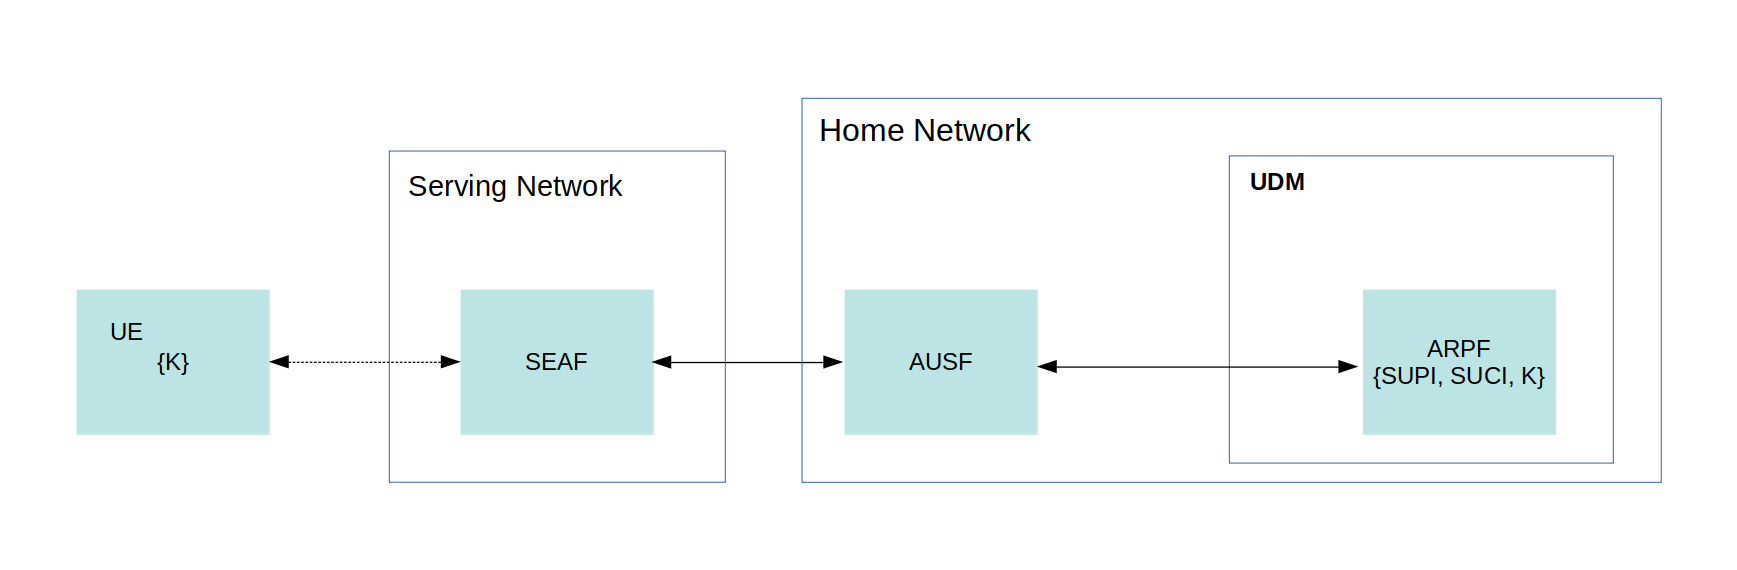
\includegraphics[scale=0.25]{Figure2_1.png}
	\end{center}
	\caption{The network components of 5G-AKA. A dotted line indicates a potentially insecure connection.}
\end{figure}

Each of these four components interacts only with the adjacent components on the list, as summarized in the high-level overview given by Figure 1. Note that we assume not only the connections within the HN but also the wired communications between SN and HN are secure. Only the wireless communication between UE and SN is considered vulnerable.

The protocol begins with an authorization request. The request can be initiated by the UE or the SEAF. Authentication can use either 5G-AKA or EAP-AKA protocol. The 5G-AKA protocol provides proof of authentication to the home network while EAP-AKA does not. 

Assuming authentication is initiated by the UE, the UE sends a N1 message to the SEAF. The message contains the UE's SUCI or 5G-GUTI. The 5G-GUTI similar to the SUCI is a temporary identifier used by the UE for over air communications. The SEAF sends a Nausf\textunderscore UEAuthentication\textunderscore Authenticate Request containing the UE SUCI or SUPI and the serving network name to the AUSF. The AUSF temporarily stores the serving network name, and determines whether the network the request was received from has the right to use that name. If the serving network name and the network the message was received from do not match, the authentication process is halted and a failure message is sent to the serving network. If the SN name and the network the message is received from agree the AUSF passes the information from the SEAF on in an Nudm\textunderscore UEAuthentication\textunderscore Get Request to the ARPF. The ARPF chooses whether EAP-AKA or 5G-AKA is used for authentication. It also determines the SUPI of the UE if the SUCI was sent in the message. 

Up to this point the process is the same for EAP-AKA and 5G-AKA. Once the determination is made which protocol to use, the two protocols diverge. In 5G-AKA ARPF generates an authentication vector, for each\\Nudm\textunderscore UEAuthentication\textunderscore Get Request received. The authentication vector consists of $<$RAND, AUTN, XRES*, $K_{ausf}$$>$. The AUTN is the AUthentication TokeN. And XRES* is the expected response from the UE. The AV is returned to the AUSF in a Nudm\textunderscore UEAuthentication\textunderscore Get Response. If the SUCI was included in the request the SUPI is included in the response. Upon receipt the AUSF stores XRES* and the SUCI or SUPI temporarily. 

The AUSF generates HXRES* which is the SHA-256 hash of XRES*. It generates $K_{seaf}$ from $K_{ausf}$. XRES* is replaced by HXRES* and $K_{ausf}$ is replaced by $K_{seaf}$ inside the AV. Before being sent in an\\Nausf\textunderscore UEAuthentication\textunderscore Authenticate Response to the SEAF, $K_{seaf}$ is removed from the AV. Once received by the SEAF, the SEAF sends RAND, and AUTN to the UE in an Authentication Request message. 

The UE determines the freshness of the AV based off the AUTN. If the AV is fresh, then it is accepted by the UE. Using USIM, the UE computes a response, RES, CK, IK. CK stands for cipher key. IK stands for integrity key. CK and IK are 128-bits and derived from K, the UE's permanent key, using RAND. 
\begin{quote}
	$CK = f_1(K||RAND) $ where $ f_1 $ is a key generating function.
	\newline
	$IK = f_2(K||RAND) $ where $ f_2 $ is a key generating function.
\end{quote} 
From RES, CK, and IK the UE computes $K_{ausf}$, $K_{seaf}$, and RES*. The UE sends a NAS Authentication Response message to the SEAF containing RES*. The SEAF computes the hash of RES* and compares it to the cached value, HRES*. If the two are the same authentication is considered successful for the serving network. The SEAF sends RES* and the SUPI or SUCI of the UE to AUSF in a Nausf\textunderscore UEAuthentication\textunderscore Authenticate Request. 

Upon receiving the Nausf\textunderscore UEAuthentication\textunderscore Authenticate Request the AUSF checks the freshness of the AV. If the AV is considered stale, then from the point of view of the home network, authentication is considered a failure. If the AV is fresh, RES* is compared to the cached value, XRES*, if the two are in agreement, authentication is considered successful for the home network. The AUSF then sends a Nausf\textunderscore UEAuthentication\textunderscore Authenticate Response message back to the SEAF indicating the result of home network authentication. If authentication was successful for the home network, the $K_{seaf}$ is included in the Nausf\textunderscore UEAuthentication\textunderscore Authenticate Response message. If a SUCI or SUPI was included in the initiating message a SUPI is also included in the response. No communication services are provided to the UE until the SEAF is given the UE SUPI. Figure 2 summarizes the transactions in a protocol diagram.

\begin{figure}[h]
	\begin{center}
		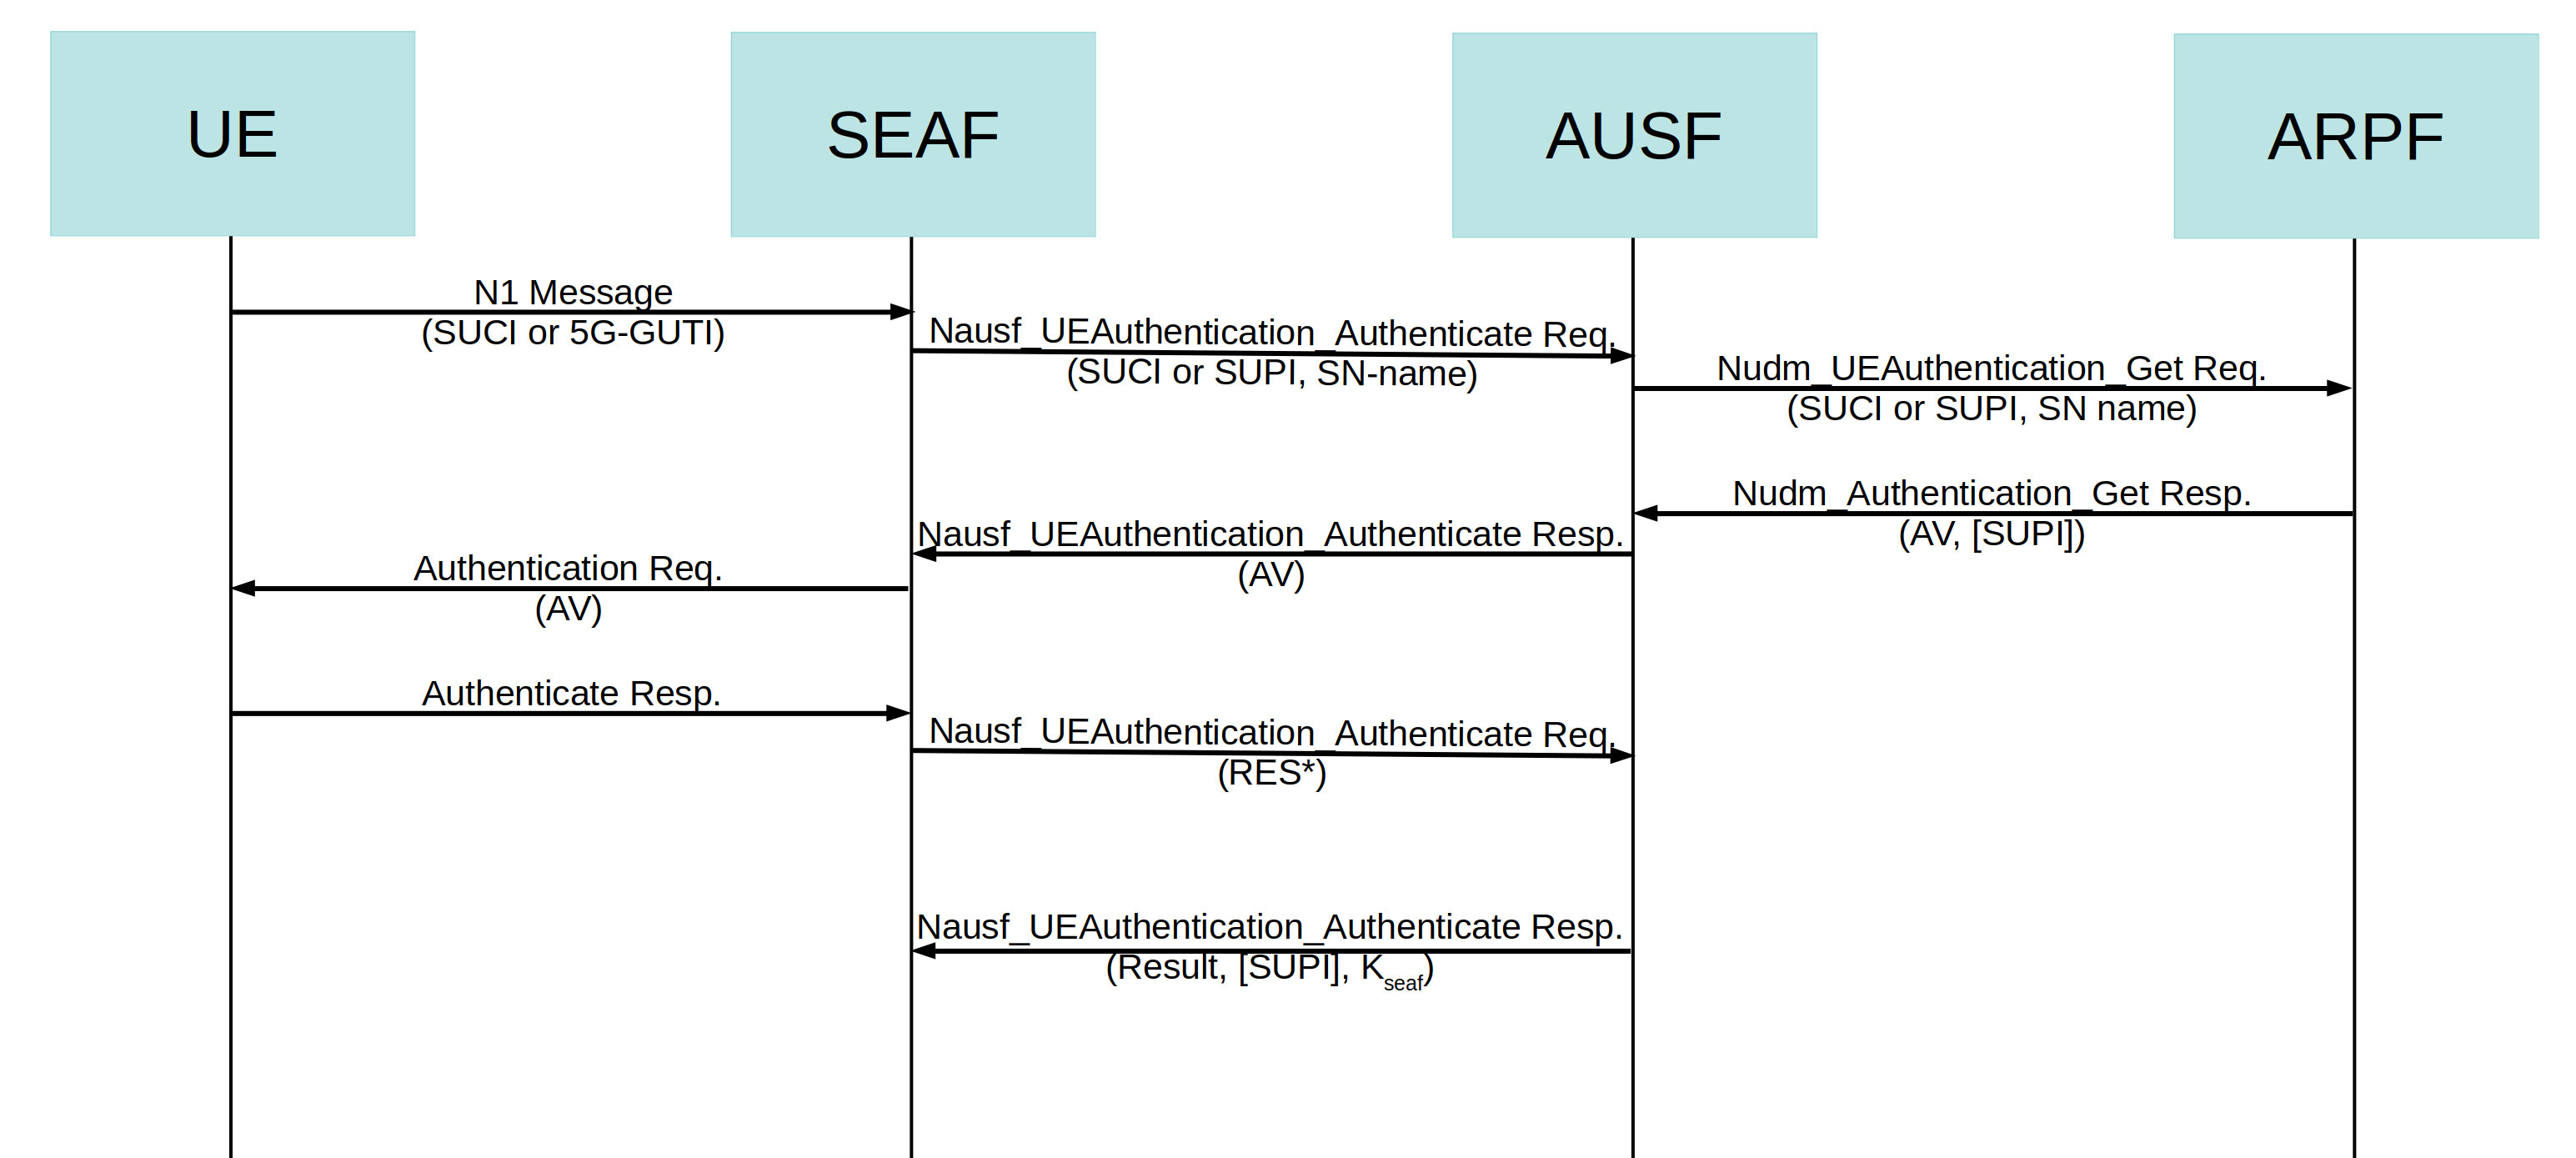
\includegraphics[scale=0.21]{Figure2_2.png}
	\end{center}
	\caption{5G-AKA protocol sequence diagram.}
\end{figure}

\subsection{Formal Verification}
Formal verification uses mathematical concepts to ensure that a security protocol fulfills its intended design. Today software based verification methods allow protocols to be systemically analyzed for flaws. There are two broad categories of verification, model checking and logical inference.\cite{edsarx.1101.181520110101} Model checking provides an exhaustive search of the model by exploration of each state and its transitions. Logical inferences is a formal mathematical verification that is seldom automated and relies on the verifier's understanding of the system. Currently model checking is the preferred method of verification. It is increasingly replacing verification by testing or simulation. 

The Tamarin prover we use in this paper falls into the model checking class of verifier. It is a symbolic modeling and analysis tool for security protocols. The verifier uses a highly specific programming language to capture the states and transitions of the protocol in combination with the Dolev-Yao adversarial model. Tamarin represents the protocol as a state machine, with the state of the system represented by a multiset of facts. Rules define state transitions. Each rule is composed of a right side, an action, and a left side, and each of these is further broken down into facts. The state is initialized to an empty multiset. A rule can only be executed if the facts on the left-side of the rule are available in the multiset. In the Tamarin language, the qualities of the protocol the tester intends to prove and written as lemmas. An example of a rule and a lemma are shown below, borrowed from an example in the Tamarin documentation.\cite{tamarinTeam}

\begin{quote}
	\begin{verbatim}
	rule Reveal_ltk:
	[ !Ltk(A, ltk) ]
	--[ LtkReveal(A) ]->
	[ Out(ltk) ]
	
	lemma Client_session_key_secrecy:
	" /* It cannot be that a */
	not(
	Ex S k #i #j.
	/* client has set up a session key 'k' with a server 'S' */
	SessKeyC(S, k) @ #i
	/* and the adversary knows 'k' */
	& K(k) @ #j
	/* without having performed a long-term key reveal on 'S'. */
	& not(Ex #r. LtkReveal(S) @ r)
	)
	"
	\end{verbatim}
\end{quote}

Each rule is named; in this case the rule is named \verb|Reveal_ltk|. The names are not used internally, however. Instead, Tamarin views rules in terms of the action facts they produce, which allows them to be associated with their arguments. This rule's action fact is \verb|LtkReveal(A)|, which takes the untyped argument \verb|A|. The action fact represents the transformation of the fact \verb|!Ltk(A, ltk)| into the fact \verb|Out(ltk)|. In particular, this fact represents an adversary being able to brute force a user's long-term key \verb|ltk|. Under the linear logic used by Tamarin, each fact can only be used once by default. However, we can mark a fact as persistent with the exclamation mark \verb|!|, such as in this case where we want the association of user \verb|A| with key \verb|ltk| to be usable multiple times. The \verb|Out(ltk)| is a special fact which broadcasts \verb|ltk|, allowing the adversary to discover \verb|ltk|.

Lemmas work using standard first-order logical notation. In this simple example, we assert that there is no combination of parameters \verb|S| and \verb|k| such that a session has been set up with server \verb|S| and key \verb|k|, the adversary knows \verb|k| (represented by the built-in \verb|K()|), and the adversary has not at some point performed long-term key reveal to discover the value of the key.

\section{Methodology}

\subsection{The Model}

As is standard in Tamarin proofs, we use the Dolev-Yao model to investigate the protocol. This approach represents a network as abstract machines which exchange messages consisting of formal terms. Because of this abstraction, it is the most straightforward way to formally examine the security properties of a network protocol.

One of the primary aspects aspect which makes the Dolev-Yao model useful for finding potential security vulnerabilities is its extremely weak assumptions about what a limits an adversary has. Any message is assumed to be completely under the control of the adversary: they can overhear, intercept, and synthesize any combination of messages subject only to their current knowledge of the network state. By giving the adversary as much power and flexibility as possible, we ensure that the model can account for as many attacks as possible, whether passive eavesdropping attacks or more active attacks involving the interception and manipulation of wireless communication.

Because of the strength of the Dolev-Yao adversary, we must be careful not to give them more strength than the 5G-AKA protocol accounts for. The purpose of 5G-AKA is to verify the interaction of the UE with the network, with all of the internal network components (SEAF, AUSF, UDM/ARPF) assumed to have secure communications with each other. This assumption includes not just integrity and authenticity but also confidentiality, since an adversary is assumed to be unable to eavesdrop on the wired communications between SN and HN. To account for this, we replace all internal messages with facts stating that a message has been sent. The adversary has no control over the facts of the experiment, and therefore can only manipulate messages between the UE and the SEAF, which is the only part of the network communicated with directly by the user. Since none of these `message facts' invoke \verb|Out|, they are also confidential. Finally, the linear logic employed by Tamarin ensures that these facts will each be used at most once, ensuring that internal messages will not be erroneously duplicated. However, to fit with the (lack of) specifications, we do not add any requirement of the ordering in which the message facts are handled by the network.

Because of the complexity of the protocol, we make certain simplifying assumptions. For example, to produce terms like HRES* our model does not implement the SHA256 algorithm specified by the protocol but instead uses Tamarin's built-in hashing theory, which is assumed to be perfectly confidential in that an adversary can deduce nothing about \verb|x| given knowledge of \verb|h(x)|. Given the robustness of SHA256, we consider this a reasonable approximation of the network's actual behavior.

\subsection{Security Properties}

There are several properties 5GAKA is intended to guarantee, encompassing both the validity of the authentication and the confidentiality of all components of the protocol which are expected to be secret, such as the user's key and SUPI. Each of the properties will correspond to a Tamarin lemma asserting that the property holds in all possible situations that might arise from the rules and for all choices the Dolev-Yao adversary may make.

Valid authentication has two components. First, we want to ensure that an adversary cannot impersonate a valid SN to a UE, authenticating with the UE without having access to an ARPF with the user's private key. Conversely, we want to ensure an adversary cannot impersonate a valid UE to the SN, again without knowing the correct private key. Each of these corresponds to a lemma of the form `if authentication is successful, then the agent in question has access to the secret key'.

To guarantee confidentiality we want to ensure that no information intended to be kept secret is leaked to an adversary, possibly including a malicious SN. One aspect of this is keeping the user's SUPI confidential. Knowledge of a user's SUPI would permit an adversary the undesirable capability of tracking a subscriber's physical location, so we want to ensure that the SUPI remains unknown to all parties involved except the user itself and the HN. For this we need two experiments. The first, modeling an outside adversary, uses the normal setup and states that the adversary never learns a user's SUPI. To model an honest but curious SN, we change the rules to produce an \verb|Out| fact whenever information is passed through the SEAF, thereby giving the adversary the same knowledge that is available to the SN.

The other aspect of confidentiality is that keys involved in the protocol (the user's long-term key \verb|K| as well as the $K_{seaf}$ and $K_{ausf}$) should remain unknown to all parties which do not need access to them. The SN needs to know the $K_{seaf}$ in order to function correctly, for example, but should not be able to deduce the user's long-term key at any point. External adversaries should not be able to deduce any keys.

Key confidentiality can be further divided into two phases. First, we want to ensure that an adversary cannot deduce secret protocol terms like $K_{seaf}$ given the ability to view normal network traffic. A second, stronger criterion is to allow the adversary to make long-term key reveals and use the information gained in order to predict new keys. We therefore again split the proof into two cases for each type of key, with one lemma to test whether an adversary can deduce the key `from scratch' and another where the adversary is allowed use of an \verb|LtkReveal| fact allowing it access to previously used keys.

\section{Setup}

The default version of the protocol is given in full in the `5gaka\textunderscore priv' theory in the appendix. We model the execution of the 5G-AKA protocol using a collection of 21 rules. Four of these provide for the creation of each of the four types of agent (UE, SEAF, AUSF, ARPF) in the 5G-AKA protocol, two associate agents with stateful features such as keys, three provide for the possibility of long-term key reveal, and the rest govern the interactions of the agents under the 5G-AKA protocol.

We also include a simplified version of the protocol, `5gaka' with the three resynchronization rules omitted. Due to the complexity of the xor operation, the Tamarin auto-prover has a tendency to `get lost' in these rules, struggling to prove that there is indeed a way for a valid user and a valid SN to authenticate with each other. Since the existence of a valid authentication is a purely existential lemma, of the form $\exists x_1, \ldots, x_n \Phi(x_1, \ldots, x_n)$, omitting rules cannot cause it to become true if it was false in the full protocol description (any trace satisfying the lemma without resynchronization rules can be exactly replicated in the case where resynchronization requests are allowed). We may therefore reason about it without the resynchronization rules, establish its validity more easily, and then know that it holds in the presence of additional rules. Other lemmas are universal rather than existential and therefore require all rules to be present in order to reason about them.

In the case of an honest-but-curious SN, we slightly modify some of the rules to have the SN output all information it receives which was not already publicly broadcast. This was given in a `5gaka\textunderscore pub' theory, so called because it makes public all information that passes through the SN. Because of its close resemblance to the default version, we do not give the full source code in the appendix but instead simply list the changes here:

\begin{itemize}
 \item The addition of an \verb|Out(<'SN_knowledge', $ausf, ~snid>)| fact in the \verb|receive_N1_message| rule.
 \item The addition of an \verb|Out(<'SN_knowledge', $ausf, hxres_star, k_seaf, ~sqnHN>)| fact in the \verb|Authenticate_Req| rule.
 \item The addition of an \verb|Out(<'SN_knowledge', suci, ~snid, $ausf>)| fact in the \verb|Nausf_final_internal| rule.
\end{itemize}

After establishing the rules of the protocol, we translate each of the security properties mentioned above into a formally stated lemma.

\section{Results}

Almost all of the security properties given above were successfully verified using Tamarin. While initial indications suggested a sophisticated attack was possible to break the given authenticity properties, a careful examination of the assumptions and correction of errors showed that no such attack existed.

Because of this verification, we have guaranteed the following properties, corresponding to the lemmas listed in the Tamarin code:

\begin{itemize}
 \item The UE will only authenticate with an SN which is in communication with an HN which knows the user's key.
 \item The SN will only authenticate with a user which provides valid evidence of holding its key.
 \item The user's SUPI remains unknown to the SN as well as all potential third-party eavesdroppers.
 \item The user's key remains unknown to the SN as well as all potential third-party eavesdroppers.
 \item The session key $K_{seaf}$ remains unknown to all potential third-party eavesdroppers.
 \item The temporary key $K_{ausf}$ constructed by the AUSF and passed to the SEAF for generation of $K_{seaf}$ remains unknown to all potential third-party eavesdroppers.
\end{itemize}

Unfortunately, the one major component we were unable to address is the possibility of past keys leaking information about future keys after long-term key reveal uncovers their values. Neither the auto-prover nor manual attempts at proof discovered either an attack or a proof of security in a reasonable amount of time (upwards of one hour of computing time on a 4-core i5 processor, after which time the computer ran out of memory and froze). Because of this, it is possible that there is a sufficiently complex attack exploiting knowledge of old keys to predict new ones.

\section{Discussion}

The significance of long-term key reveals is unclear in the 5G context. While it would be significant to discover an attack allowing the prediction of new session keys based on old ones, long-term key reveal poses a problem for 5G-AKA for other reasons. Security-essential components like the UE's key and SUPI are constant. If we assume an adversary can eventually determine an old $K_{seaf}$, it is also reasonable to assume they might determine an `old' UE key or SUPI. But because these values are constant, this would immediately break the 5G-AKA protocol. If an adversary ever learns the UE's key, they can perfectly impersonate a legitimate SN. Long-term key reveal therefore poses potential problems even beyond the scope of the concerns addressed in the 5G-AKA communication, since key network components may be kept in use indefinitely.

Furthermore, while we have addressed the security properties of 5G-AKA, some questions remain. As pointed out by Basin et al,\cite{basin2018formal} the security of 5G-AKA is closely related to that of other protocols in the 5G suite. For example, the possibility of an SN initiating `key change on-the-fly' could potentially allow an adversary to hijack communications by requesting a key change immediately after the 5G-AKA protocol has been followed.

Other vulnerabilities may be possible because of the simplifying assumptions the model makes. An approach which abstracts away fewer cryptographic details may uncover a vulnerability which this verification missed. The use of several different key-generating functions, all assumed here to be perfectly secure, complicates the potential analysis significantly, especially when values are combined using operations like xor. Even in our analysis, the difficulty of providing guarantees about this operation produced significant overhead in proving the security lemmas.

Finally, we stress that formal analysis is not the only approach which should be taken in analyzing any component of a protocol. Figuring out whether a real-world system correctly implements a protocol can be a difficult undertaking, and a failure to comply with the protocol may not be noticed until an adversary discovers a vulnerability.

\section{Conclusion}

With 5G promising to become the new standard for mobile communication, it is important that its security properties be tested thoroughly. In particular, the 5G-AKA protocol forms the first key component in ensuring authenticity and privacy from adversaries. Using the Tamarin prover, we have modeled the 5G-AKA protocol and tested several important security properties. This model shows that the authentication properties of the protocol are correct, once currently-known vulnerabilities are accounted for. Furthermore, several privacy properties hold as well, so that 5G-AKA is shown to provide protection against tracking users via SUPI and similar attacks. However, long-term key reveal still poses a potential threat to authentication security.

\nocite{*}
\bibliography{References}
\bibliographystyle{plain}

\appendix
\section{Tamarin Code}

\begin{quote}
	\begin{verbatim}
theory 5gaka_priv
begin

builtins: hashing, xor

rule create_ue:
		let
			suci = h(~supi, $hn)
		in
		[Fr(~supi), Fr(~K), Fr(~sqnUE)]
	--[AssignUserID($ue, ~K, suci, ~supi)]->
		[!UE_Identity($ue, suci, ~supi, ~sqnUE, $hn), !LongTermKey($ue, ~K),
		Out(suci), Out($hn)]

rule create_seaf:
		[Fr(~snid)]
	-->
		[!SEAF_Identity($seaf, ~snid)]

rule create_ausf:
		[]
	-->
		[!AUSF_Identity($ausf)]

rule create_arpf:
		[]
	-->
		[!ARPF_Identity($arpf)]

rule assoc_ue_hn:
		[!UE_Identity($ue, suci, ~supi, ~sqnUE, $hn), !LongTermKey($ue, ~K),
		!ARPF_Identity($arpf)]
	--[KeyReveal($arpf, $ue, ~K)]->
		[!ARPF_Store_Info($arpf, $ue, ~supi, ~K)]

rule init_sqn:
		[!UE_Identity($ue, suci, ~supi, ~sqnUE, $hn), !AUSF_Identity($ausf),
		Fr(~sqnHN)]
	-->
		[!AUSF_Store_Info($ausf, $ue, ~sqnHN)]

rule Reveal_k:
		[!UE_Identity($ue, suci, ~supi, ~sqnUE, $hn),
		!ARPF_Store_Info($arpf, $ue, ~supi, ~K)]
	--[LtkReveal($ue, ~K)]->
		[Out(~K)]

rule Reveal_k_seaf:
		[!Stored_Keys($ue, $ausf, k_seaf, k_ausf)]
	--[Ltk_seafReveal($ue, k_seaf)]->
		[Out(k_seaf)]

rule Reveal_k_ausf:
		[!Stored_Keys($ue, $ausf, k_seaf, k_ausf)]
	--[Ltk_ausfReveal($ausf, k_ausf)]->
		[Out(k_ausf)]

rule N1_message:
        [!UE_Identity($ue, suci, ~supi, ~sqnUE, $hn),
        !SEAF_Identity($seaf, ~snid)]
    --[SendN1($ue, $seaf)]->
    	[Out(<'N1_message', $ue, $seaf, suci, $hn>)]

rule receive_N1_message:
        [!SEAF_Identity($seaf, ~snid), !AUSF_Identity($ausf),
        In(<'N1_message', $ue, $seaf, suci, $hn>)]
    -->
       	[Nausf_UEAuthentication_Authenticate_Request($seaf, $ausf, suci,
       	$hn, ~snid)]

rule Nausf_UEAuthentication_Authenticate_Req:
        [!SEAF_Identity($seaf, ~snid), !AUSF_Identity($ausf),
        !ARPF_Identity($arpf),
        Nausf_UEAuthentication_Authenticate_Request($seaf, $ausf, suci,
        $hn, ~snid)]
    -->
    	[Ndm_UEAuthentication_GET_Request($ausf, $arpf, suci, ~snid)]

rule Ndm_UEAuthentication_GET:
		let
			xres_star = h(~K, ~snid, ~rand)
			k_ausf = h(~K, ~snid)
		in
        [Fr(~rand), !ARPF_Identity($arpf), !ARPF_Store_Info($arpf, $ue,
        ~supi, ~K), !UE_Identity($ue, suci, ~supi, ~sqnUE, $hn),
        Ndm_UEAuthentication_GET_Request($ausf, $arpf, suci, ~snid)]
    --[SetupKausf($ausf, ~supi, k_ausf)]->
    	[!StoreRand($arpf, ~supi, ~rand),
    	Ndm_UEAuthentication_GET_Response($arpf, $ausf, ~rand, ~supi, ~snid,
    	xres_star, k_ausf)]

rule Nausf_UEAuthentication_Authenticate_Resp:
		let
			hxres_star = h(~rand, xres_star)
			k_seaf = h(k_ausf, ~snid)
		in
		[!AUSF_Identity($ausf), !SEAF_Identity($seaf, ~snid),
		!AUSF_Store_Info($ausf, $ue, ~sqnHN),
		Ndm_UEAuthentication_GET_Response($arpf, $ausf, ~rand, ~supi, ~snid,
		xres_star, k_ausf)]
	--[StoreXRES($ausf, xres_star, hxres_star)]->
		[StoredXRES($ausf, xres_star, hxres_star),
		!Stored_Keys($ue, $ausf, k_seaf, k_ausf),
		Nausf_UEAthentication_Authenticate_Response($ausf, $seaf, ~rand,
		hxres_star, k_seaf, ~sqnHN)]

rule Authenticate_Req:
		[!SEAF_Identity($seaf, ~snid),
		!UE_Identity($ue, suci, ~supi, ~sqnUE, $hn),
		Nausf_UEAthentication_Authenticate_Response($ausf, $seaf, ~rand,
		hxres_star, k_seaf, ~sqnHN)]
	--[SetupKseaf($ue, $seaf, k_seaf)]->
		[Out(<'Authentication_Request', $seaf, ~snid, $ue, ~rand, ~sqnHN>)]

rule Resync_request:
		[!UE_Identity($ue, suci, ~supi, ~sqnUE, $hn),
		!ARPF_Store_Info($arpf, $ue, ~supi, ~K),
		!SEAF_Identity($seaf, ~snid),
		In(<'Authentication_Request', $seaf, ~snid, $ue, ~rand>)]
	-->
		[Out(<'Sync_failure', $ue, ~sqnUE XOR h(~K, ~rand),
		h(~K, ~sqnUE, ~rand)>)]

rule Resync_forward_hn:
		[!SEAF_Identity($seaf, ~snid), !AUSF_Identity($ausf),
		In(<'Sync_failure', $ue, ~sqnUE XOR h(~K, ~rand),
		h(~K, ~sqnUE, ~rand)>)]
	-->
		[ResyncRequest($ue, $ausf, ~sqnUE XOR h(~K, ~rand),
		h(~K, ~sqnUE, ~rand))]

rule Resync_process:
		[!AUSF_Identity($ausf), !ARPF_Identity($arpf),
		!StoreRand($arpf, ~supi, ~rand),
		!ARPF_Store_Info($arpf, $ue, ~supi, ~K),
		ResyncRequest($ue, $ausf, resync_val, h(~K, ~sqnUE, ~rand))]
	-->
		[!AUSF_Store_Info($ausf, $ue, resync_val XOR h(~K, ~rand))]

rule Authenticate_Resp:
		let
			res_star = h(~K, ~snid, ~rand)
		in
		[!UE_Identity($ue, suci, ~supi, ~sqnUE, $hn),
		!ARPF_Store_Info($arpf, $ue, ~supi, ~K),
		!SEAF_Identity($seaf, ~snid),
		In(<'Authentication_Request', $seaf, ~snid, $ue, ~rand>)]
	--[AuthResponse($ue, $seaf, $arpf)]->
		[Out(<'Authentication_Response', $seaf, ~snid, $ue, suci,
		res_star, ~rand>)]

rule Nausf_final:
		let
			hres_star = h(~rand, res_star)
		in
		[!SEAF_Identity($seaf, ~snid), !AUSF_Identity($ausf),
		StoredXRES($ausf, xres_star, hres_star),
		In(<'Authentication_Response', $seaf, ~snid, $ue, suci,
		res_star, ~rand>)]
	--[AuthSuccess($ue, $seaf, $ausf)]->
		[Nausf_UEAuthentication_Authenticate_Response(suci, $seaf,
		~snid, $ausf)]

rule Nausf_final_internal:
		[!SEAF_Identity($seaf, ~snid), !AUSF_Identity($ausf),
		StoredRES($ausf, hres_star),
		Nausf_UEAuthentication_Authenticate_Request(res_star, suci, $seaf,
		~snid, $arpf)]
	--[ReportAuthSuccess($seaf, $ausf, suci)]->
		[Nausf_UEAuthentication_Authenticate_Response(suci, $seaf,
		~snid, $ausf)]

lemma Valid_setup:
	exists-trace
	" Ex ue key suci supi seaf ausf #i #j #k.
		AssignUserID(ue, key, suci, supi) @ #i
		& SendN1(ue, seaf) @ #j
		& AuthSuccess(ue, seaf, ausf) @ #k
		& #i < #k
	"

lemma Auth_seaf_legit:
	" All ue key suci supi seaf ausf #i #j #k.
		(SendN1(ue, seaf) @ #i
		& AssignUserID(ue, key, suci, supi) @ #j
		& ReportAuthSuccess(seaf, ausf, suci) @ #k)
		==>
		(Ex arpf k #r. KeyReveal(arpf, ue, k) @ #r)
	"

lemma Auth_client_legit:
	" All ue suci seaf ausf #i #j.
		(SendN1(ue, seaf) @ #i
		& ReportAuthSuccess(seaf, ausf, suci) @ #j)
		==>
		(Ex key supi #r. AssignUserID(ue, key, suci, supi) @ #r)
	"

lemma SUPI_private:
	" All ue key suci supi #i.
		((AssignUserID(ue, key, suci, supi) @ #i)
		==>
		not (Ex #j. K(supi) @ #j))
	"

lemma User_key_private:
	" All ue k suci supi #i #j.
		(AssignUserID(ue, k, suci, supi) @ #i
		& K(k) @ #j
		==>
		(Ex #k. LtkReveal(ue, k) @ #k))
	"

lemma K_SEAF_private:
	" All ue seaf k #i #j.
		(SetupKseaf(ue, seaf, k) @ #i
		& K(k) @ #j
		==>
		(Ex user #k. Ltk_seafReveal(user, k) @ #k)
		| (Ex ausf k2 #k. Ltk_ausfReveal(ausf, k2) @ #k)
		| (Ex user k2 #k. LtkReveal(user, k2) @ #k))
	"

lemma K_AUSF_private:
	" All suci ausf key #i #j.
		(SetupKausf(ausf, suci, key) @ #i
		& K(key) @ #j
		==>
		(Ex ausf2 k2 #k. Ltk_ausfReveal(ausf2, k2) @ #k)
		| (Ex user k2 #k. LtkReveal(user, k2) @ #k))
	"

end
	\end{verbatim}
\end{quote}

\end{document}